\section{Neue Medien - AH}
\textit{Autor: Aurelian Hermand}


Hochschultrends in den neuen Medien umfassen den online Auftritt bezüglich der Erstellung, Verarbeitung und Bereitstellung von Informationen und ferner die ganzheitliche Außendarstellung mittels Marketing. Die Imagebildung der Hochschulen folgt dabei festgelegten Prinzipien und Zielen. Marketing kann nicht leicht abgegrenzt werden, denn man kann nicht nicht kommunizieren. Von der serviceorientierten und prozessorientierten Organisationsstruktur der Hochschule bis hin zum direkten Online-Marketing über den Webauftritt und soziale Plattformen werden Studenten und Hochschulangehörigen konfrontiert mit neuen Medien. Im Zuge der Consumerisation haben sich die Grenzen der Nutzung von privater und beruflicher Software und Geräte aufgelöst. Eine homogen gestaltete Infrastruktur ist damit hinfällig. Der Trend zum BYOD (Bring Your Own Device) hat veranlasst, dass eine Infrastruktur flexibel gestaltet wird und werden muss. Insbesondere auch die gestiegene Nutzung von Mobilgeräten wie Smartphones und Tablets dazu geführt, dass Software neuen Vorgaben gerecht werden muss.


\subsection{Infrastruktur und Management}
Im folgenden werden Trends im Bezug auf die Infrastruktur an Hochschulen und im speziellen an der Hochschule Emden / Leer betrachtet. 

\subsubsection{Netzinfrastruktur, Consumeration und BYOD}
\label{netzinfrastruktur_consumeration_und_byod}
Viele Hochschulen in Europa haben sich mittlerweile dem Projekt eduroam (education roaming) angeschlossen. Eduroam ermöglicht die Nutzung von WLAN und LAN an jeder teilnehmenden Hochschule durch vorherige Authentifizierung mit den erhaltenen Zugangsdaten.

Eduroam als standardisierte Lösung macht die Teilnahme verschiedenster Geräte und Standorte im Zuge der Consumeration und BYOD sehr einfach. Geringere Support-Aufwendungen auf der anderen Seite ermöglichen es die Serviceorientierung teilweise abzulösen und durch Prozessorientierung zu ersetzen. Der Aufwand erhöht sich jedoch für die Administratoren durch "die Offenheit der Gerätewahl"\footnote{\url{http://www.wickhill.de/theguardian/byod-viele-vorteile-bei-einhaltung-von-sicherheitsspielregeln/}}, wobei der Sicherheitsaspekt hier eine große Rolle spielt. An den Standorten selber kommt es in Folge der Offenheit für die Benutzer wiederum so zur Steigerung der Produktivität und Benutzerzufriedenheit. Die Arbeitsabläufe werden hierdurch flüssiger und effizienter.

\subsubsection{Software für Forschung und Lehre}
Das Netzwerk Dreamspark ermöglicht es Studenten und Bedienstete im Rahmen von Forschung und Lehre kostenlos eine Vielzahl von Microsoft Softwareprodukten zu erhalten und auf Ihren Geräten zu installieren.

Die Hochschulen Osnabrück und Hannover, wie auch die Hochschule Emden / Leer ermöglichen die Teilnahme.

Der Service kann mit Hinweisen auf kostenlose Software für Forschung und Lehre erweitert werden. So bietet JetBrain  ebenfalls ein Teil seiner Software kostenlos Studenten an \footnote{\url{https://www.jetbrains.com/student/}}. Ebenfalls bietet auch GitHub ein Paket für Studenten \footnote{\url{https://education.github.com/}}.


\subsubsection{Identitätsmanagement}
Ein umfassendes Identitätsmanagement setzt eine komplexe Architektur voraus. Die zwei Hauptfunktionen des Identitätsmanagement klassifiziert sich in:

\begin{itemize}
  \item Neuen Benutzern
  \item Entfernung von Benutzern \ldots
\end{itemize}


Verfolgt wird der Trend, die Einrichtung und Löschung schnell und zentral erledigen zu können. Dabei keinen Benutzer-Daten klar und nachvollziehbar zu hinterlegen. \footnote{\url{https://www.rrzn.uni-hannover.de/fileadmin/it_sicherheit/pdf/SiTaWS08-idm.pdf}}

Die Einmalanmeldung (Single-Sign-On) ermöglicht dem Benutzer alle angeschlossenen Dienste einer Hochschule zu nutzen, ohne sich mehrfach Authentifizieren zu müssen. An der HS Emden/Leer wird dabei auf Shibboleth gesetzt. 

\subsubsection{E-Mail}
Ein integraler Bestandteil an Hochschulen ist der E-Mail Service. Der Trend geht zu einem zentralen System für Mitarbeiter und Studenten. Im Sinne des Consumeration ist die Nutzung des E-Mail Service offen gestaltet für alle vorstellbaren Endgeräte und Programme. Zudem gibt es Webmailer um auch von Fremdrechnern an die E-Mails zu gelangen.

\subsubsection{E-Learning Plattform}
\label{subsubsection_e_learning_plattformen}
Das elektronische Lernen setzt auf den Einsatz von digitaler Medien.
Das Blended Learning vereint 3 Lerndomänen, das lernen online durch Kommunikation, Distanziert ohne Interaktion und in der Präsenz. Auch im Präsenzstudium wird zunehmend nicht nur auf offline Medien Skripte oder Bibliothek gesetzt, sondern auch auf online Abgaben, Aufzeichnung, Videochats und Foren.

Dazu gibt es zwei größere Plattformen ILIAS und Moodle. Die Hochschule setzt Moodle ein, dass jedoch weitgehend nicht verpflichtend im Präsenzstudium ist. Als Angebot könnten, wie im Online-Studium Skripte zur Verfügung gestellt und weiterentwickelt werden, welches die Lehrenden übernehmen verwenden können. Der Vorteil liegt darin, dass um ein Skript herum ein Ökosystem aus Übungsaufgaben, Videos und Beiträgen entsteht.


\subsection{Dokumentenverwaltung}
Die Dokumentenverwaltung umfasst verschiedene Services, da die Anforderungen sehr unterschiedlich sind.


\subsubsection{Wiki}
Das Wiki ist ein Dienst zur Erfassung ungeordneter, miteinander verknüpfbarer Texte. Sie sind sehr flexibel einsetzbar. Es lassen sich Informationen schnell, versionsbasiert gemeinsam zusammentragen.

Wikis stellen oft die Basis für Informationsverwaltungen, aus denen konzentriertere Informationssysteme entstehen können in Form von Websites oder auch FAQs, Anleitungen uvm.



\subsubsection{Clouds und Big Data}
Clouds ermöglichen den einfachen Datenaustausch großer Dateien mit verschiedenen Zugriffsrechten. Eingeteilt werden können die Clouds in


\begin{itemize}
  \item Öffentliche Clouds
  \item Private Clouds
  \item Hybride Clouds
  \item Community Clouds \ldots
\end{itemize}

Die Community Cloud stellt einem definierten Nutzerkreis von mehreren Standorten Zugriff auf die Cloud zur Verfügung. Hierbei wird gemeinsam oder von einem Anbieter die die Cloud verwaltet. Die Hochschulen in NRW als Verbund setzen auf diese Cloud-Form. Dahinter steckt die Software ownCloud. Die Lösung nennt sich Sciebo die CampusCloud.

Die Hochschule Emden / Leer führt derzeit mit Hilfe des Shibboleth-Dienstes eine Cloud namens „Gigamove“ zum Austausch großer Datenmengen ein. Gigamove wird von der RWTH Aachen zur Verfügung gestellt \footnote{\url{https://gigamove.rz.rwth-aachen.de}}. Die Spezifikationen dieser Cloud erlauben es Bediensteten der Hochschule 10 GByte mit Personen / Institutionen auszutauschen. Dabei ist es Möglich Dateien anderen zur Verfügung zu stellen, als auch anderen Platz einzuräumen. Nach 14 Tagen werden die Daten automatisch gelöscht und ist daher eine Austauschplattform und kein Massenspeicher.

\subsubsection{Versionsverwaltung}
Die Versionsverwaltung dient allgemein zur Dokumentenerstellung, -bearbeitung und -verwaltung. Dabei ist es jederzeit möglich auf einen vorhergehenden Stand zurückzusetzen oder Änderungen nachvollziehen zu können, damit auch ein gemeinsames Arbeiten an einem Dokument möglich ist. Die Uni Kassel setzt auf das DMS (Dokumentenmanagement) Alfresco. Alfresco ist ein bequemes und unkompliziertes System mit dem verschiedene Dokumente und Dateien zentral verwaltet werden können. Diese Software bietet Features wie Benutzerverwaltung, Integration in Moodle, Workflows zur Dokumentenüberprüfung, Aufgabenverteilung, Zusammenfassung, Versionierung von Office- oder PDF-Dokumenten. Außerdem steht eine App für Mobilgeräte bereit.\footnote{\url{http://www.uni-kassel.de/its-handbuch/kommunikation/dms/dokumentenmanagement-dms.html}}


\subsubsection{Zentrales Druckzentrum}
Das ZIV (Zentrum für Informationsverarbeitung) der Uni Münster zentralisiert u.a. die Rechnerräume, aber unterhält auch ein Druckzentrum. Das Druckzentrum bietet den Service von zu Hause zu drucken, dies schließt den Mobilgeräte ein. Die Drucke landen in einem zugeordneten Postfach mit einem farbigen Deckblatt und können von dort zu einem späteren Zeitpunkt aus dem Fach genommen werden können.
\footnote{\url{https://www.uni-muenster.de/imperia/md/content/ziv/pdf/printpay_flyer.pdf}}

\subsection{Außendarstellung und Marketing Instrumente}
Das Marketing und die Präsentation der Hochschule erfolgt breit gefächert und geht im Idealfall fließend ineinander über. Die Trends erfolgen oft in Organisatorischen Maßnahmen \footnote{\url{http://www.dfg.de/download/pdf/dfg_im_profil/gremien/hauptausschuss/it_infrastruktur/dfg_tum_bode.pdf, S.4f.}}. D.h. es wird am Ausbau und Vereinheitlichung gearbeitet, im Sinne von Corporate Identity bzw. Corporate Design der Webdienste, E-Learning Plattform, zentrale Datenspeicher, Verwaltungs EDV und sonstigen Angeboten.

\subsubsection{Website}
Die Website ist ein integraler Bestandteil der Hochschulen. Alle relevanten Informationen werden hierfür aufbereitet und dem Benutzer zugänglich gemacht. Der technische Fortschritt, verlangt zudem Beachtung neuer Designkriterien um die Sichtbarkeit im Internet zu gewährleisten.

\paragraph{Responsive Website}\mbox{}\\ % <-- bei Verwendung des Paragraph-tags bitte beachten.
Responsivität im Webdesign heißt, dass im Sinne des BYOD, der Zugriff auf die Hochschul-Website komfortabel und geräteunabhängig gestaltet ist. Die Fachhochschulen Köln und Münster sind dem Trend gefolgt, jedoch ohne auf einen etablierten Marktstandard zu setzen.

Es gibt zwei sehr verbreitete Frameworks, die meist aus Sammlungen von Modulen, Grids und Best-Practices bestehen, wie dem Prinzip des Mobile First. Mobile First bedeutet, dass aus Gründen des meist kleineren Bildschirms der Fokus auf den Inhalt liegt. Hiermit wird auch gleichzeitig das Prinzip des "Content First" bzw. "User First" umgesetzt. Sowohl Bootstrap von Twitter als auch Foundation von Zurb gelten als ausgereifte Frameworks. Die Verständigung auf ein ausgereiftes System, kann eine kostenintensive und proprietäre Selbstentwicklung verhindern. Twitter Bootstrap wird bspw. von der Hochschule Coburg und der TU München eingesetzt.

Die responsive Umsetzung mit Mobile First erhöht deutlich die Gebrauchstauglichkeit (engl. Usability), weil die Website auf dem Mobilgerät nicht gezoomt werden muss und so ausgeliefert wie der Designer es konzipiert hat. 

Die neueste Entwicklung im Bereich responsive Umsetzung erfolgte durch die Änderung des Such-Algorithmus von Google im April 2015. Die Änderung betrifft die Bewertung mobil optimierte Websites in den Suchergenissen, die fortan bevorzugt behandelt werden, sofern über ein Mobilgerät gesucht wird.

\paragraph{Sichtbarkeit und SEM}\mbox{}\\ % <-- bei Verwendung des Paragraph-tags bitte beachten.
Das Suchmaschinen-Marketing wird zusammengefasst unter dem Kürzel SEM (Search-Engine-Marketing). SEM umfasst die Konzepte SEO (Search-Engine-Optimization) und das SEA (Search-Engine-Advertising). \footnote{\url{B2B-Online-Marketing und Social Media, S.83}}

Die Suchmaschinen-Werbung bzw. SEA wird genutzt um gezielt bestimmte Suchbegriff gegen Bezahlung auf den ersten Seiten der Suchmaschinen als Werbung einzublenden.

Darunter SEO versteht man die allgemeine Suchmaschinen-Optimierungs-Maßnahmen, um im organischen Ranking weit vorne zu landen.

Der Sichtbarkeitsindex dient als Indikator für die Sichtbarkeit einer Website im Google Ranking. Dabei errechnet sich der Index aus:


\begin{itemize}
  \item dem Ranking der thematisch überwachten Keywords
  \item dem zu erwartenden Traffic aus der Positionierung und
  \item dem zu erwartenden Traffic aus dem Keyword. \ldots
\end{itemize}

Der Sichtbarkeitsindex wird als ein weiterer Messwert herangezogen für den Erfolg von SEO-Maßnahmen, neben u.a. Zugriffszahlen und Verweildauer der Besucher. \footnote{\url{https://de.onpage.org/wiki/Sichtbarkeitsindex}}

Die www.hs-emden-leer.de erreicht laut SISTRIX im Mai 2015 einen Sichtbarkeitsindex von 0,31. Im Vergleich dazu erreicht www.hs-coburg.de 0,62 und www.jade-hs.de 0,69. \footnote{\url{http://www.sichtbarkeitsindex.de/}} Die Hochschule Emden / Leer hat demnach noch Potential nach oben.

\paragraph{Inhaltsaufbereitung}\mbox{}\\ % <-- bei Verwendung des Paragraph-tags bitte beachten.
Der wichtigste Teil einer Website ist der Inhalt selber, der Fokus hierin liegt auf Vollständigkeit und einer verständlichen Sprache. Die Inhalte werden Aufbereitung und andere Ausgabemedien, wie zum Beispiel in sozialen Medien, PDFs, Drucklayouts, XML-Sitemaps und RSS ausgegeben.

RSS ist ein XML-Format zur Übertragung vorallem von News und Informationen. Die HS Emden/Leer setzt RSS an vielen Stellen ein, wie dem InfoSys und den nächsten Terminen.

\subsubsection{Social Media}
"Social-Media-Marketing (SMM) ist eine Form des Online-Marketings, die Branding- und Vertriebsziele durch ein Engagement in einem oder in verschiedenen sogenannten Social- Media-Angeboten erreichen will." \footnote{\url{Praxiswissen Online-Marketing - S.31}}

Newsletter Kampagnen sind ein trotz vieler neuer Medien weiterhin ein wichtiger Baustein im Online-Marketing-Mix. Es gibt einen klaren Trend in Richtung hin zu Mobilgeräten. Die Öffnungsraten auf mobilen Endgeräten sind seit 2010 bis 2013 um 300 Prozent angestiegen und übertreffen mittlerweile auch die Öffnungsraten der gewöhnlichen Desktop-Geräte. Betreiber des E-Mail-Marketing setzen umso mehr auf die Optimierung der Kampagnen auf mobile Endgeräte \footnote{\url{Praxiswissen Online-Marketing - S.35}}. Um den Wiedererkennungseffekt zu fördern und die eigene Marke zu etablieren, sollte beim Marketing auf das Corporate Design gesetzt werden.

Dem Social-Media-Marketing stehen unzählige weitere Vertriebskanäle zur Verfügung, wie Facebook, Twitter oder YouTube. Wichtig ist dabei vorher ein Leitbild zu entwickeln und beizubehalten. \footnote{\url{http://www.hs-merseburg.de/fileadmin/_migrated/content_uploads/090219_Marketingkonzept_Final.pdf S.8}}

\begin{figure}[h!]
	\centering
	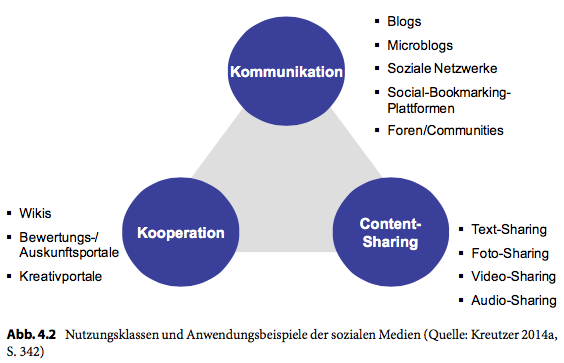
\includegraphics[width=10cm]{kapitel/gruppe1_2/bilder/nutzungsklassen}
	\caption{Nutzungsklassen und Anwendungsbeispiele sozialen Medien (Quelle: B2B Online-Marketing und Social Media, S. 152)}
	\label{fig_nutzungsklassen}
\end{figure}

Die Soziale Medien können auf vielfältige Weise genutzt werden. Die Nutzungsklassen, siehe Abbildung \ref{fig_nutzungsklassen} der sozialen Medien können in drei Bereiche aufgeteilen werden:


\begin{itemize}
  \item Kommunikation: Blogs, Microblogs, Soziale Netzwerke, Social-Bookmarking-Plattformen, Foren/Communities
  \item Content-Sharing: Text, Foto, Video, Audio
  \item Kooperation: Wikis, Bewertungs-/Auskunftsprotale, Kreativportale \ldots
\end{itemize}

Die Nutzungsklasse \ref{fig_nutzungsklassen} "Kommunikation" zielt darauf ab, aufbereitete Informationen über private und professionelle Netzwerke bereitzustellen und zu diskutieren.
Ähnlich der Nutzungsklasse "Kommunikation" zielt auch das "Content-Sharing" darauf Inhalte zu teilen über spezifische Media-Sharing Plattformen.
Bei der Nutzungsklasse "Kooperation" steht vorallem die gemeinsame Aufbereitung von Informationen im Mittelpunkt.

Social Media spielt für die Rekrutierung neuer und Erreichbarkeit bestehender HS-Interessierter eine wichtige Rolle. Hierüber können Angebote, Stellenausschreibungen geschehen. Diese können dann verlinkt und geteilt werden. 

Eine Integration in die Website sollte Datenschutzrechtlich vorgenommen werden, bspw. mit der 2-KLick-Technik.


\subsubsection{App als Informationssystem}
Der Trend geht zu Informationssystemen in Apps. Ein allgemeiner Trend dabei ist das Prinzip die Apps sowohl offline als auch online Verfügbar zu gestalten (Offline First).

\begin{figure}[h!]
	\centering
	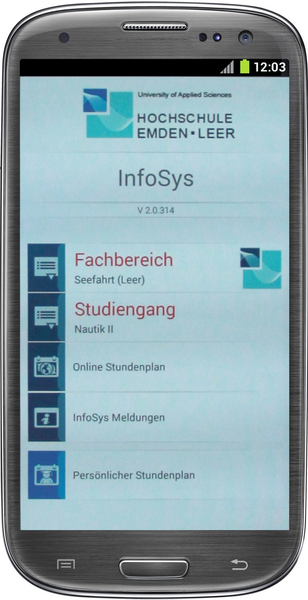
\includegraphics[width=10cm]{kapitel/gruppe1_2/bilder/hsel-androidapp}
	\caption{Android App der HS Emden / Leer}
	\label{fig_hselandroidapp}
\end{figure}

Die Hochschule Emden / Leer ist dem Trend gefolgt und hat Anfang 2014 eine Android App im Rahmen einer Projektarbeit vorgestellt, siehe Abbildung \ref{fig_hselandroidapp}. Das Prinzip "Offline First" wurde dabei berücksichtigt. Hauptaugenmerk wurde dabei auf die Integration von InfoSys und die Individualisierungssmöglichkeiten der Studentenden gelegt, um den Stundenplan anzupassen. \footnote{\url{http://www.hs-emden-leer.de/aktuelles-termine/news/article/immer-up-to-date-dank-neuem-smartphone-app.html}}

Da die Entwicklung im Rahmen einer Projektarbeit vonstatten ging, wird es sehr wahrscheinlich bei dieser einen Version und dem einzigen Gerätetyp bleiben.

\begin{figure}[h!]
	\centering
	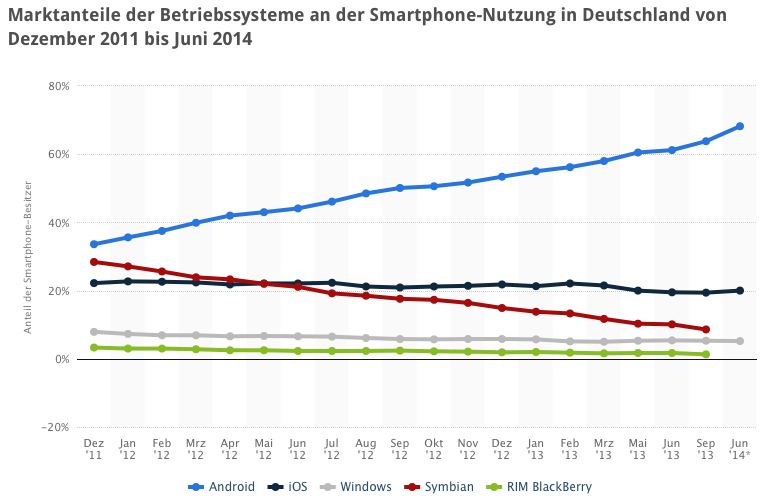
\includegraphics[width=10cm]{kapitel/gruppe1_2/bilder/marktanteile}
	\caption{Marktanteile der Betriebssysteme an der Smartphone-Nutzung in Deutschland von 2011 bis 2014}
	\label{fig_marktanteile}
\end{figure}
\footnote{\url{http://de.statista.com/statistik/daten/studie/170408/umfrage/marktanteile-der-betriebssysteme-fuer-smartphones-in-deutschland/} Statista, 2014}

An Hand der Marktanteile \ref{fig_marktanteile} werden u.a. 20 Prozent iOS Nutzer nicht berücksichtigt und ist nicht im Sinne von BYOD, da eine Beschränkung vorliegt. Der Grund dafür liegt an den Unterschieden der Betriebssysteme. Für jedes System muss prinzipiell eine eigene App entwickelt werden. Ein kostengünstiger Lösungsansatz ist der Einsatz ausgereifter Javascript Webapp-Frameworks, wie beispielsweise Sencha Touch und AngularJS. Die Apps lassen sich so mit jedem Gerät zunächst einmal als Website auf dem Mobilgerät öffnen und mit Hilfe von Cordova/Phonegap ist es weiterhin möglich diese Webapps in den wichtigsten App Stores auszuliefern.

Nicht nur Flexibilität im Bezug auf Geräteunabhängigkeit wird geschaffen, auch Hürden der Weiterentwicklung werden verringert, da auf ausgereifte Software gesetzt wird.


\paragraph{InfoSys und News}\mbox{}\\ % <-- bei Verwendung des Paragraph-tags bitte beachten.
An einigen Hochschulen, wie der Hochschule Heidelberg werden u.a. Hochschulinformationen und Aktuelle Nachrichten direkt über eine App ausgeliefert. Die Integration des InfoSys und der aktuellen Nachrichten der Hochschule sind vorhanden, jedoch existieren diese Informationen nur für Android Benutzer.

\paragraph{HIS (Notenzugriff, Stundenpläne)}\mbox{}\\ % <-- bei Verwendung des Paragraph-tags bitte beachten.
Die HAW Hamburg und auch die Hochschule Heidelberg ermöglicht in der App den Zugriff auf Stundenpläne, Raumpläne, Prüfungen und Noten \footnote{\url{https://itunes.apple.com/de/app/haw-hamburg/id670347114?mt=8}}. Die Hochschule Emden / Leer hat in der Android App nur den Zugriff auf die Stundenpläne. Ableiten lässt sich daraus, dass geprüft werden muss, ob das HIS, den Zugriff über eine Schnittstelle ermöglicht.

\paragraph{Mensa}\mbox{}\\ % <-- bei Verwendung des Paragraph-tags bitte beachten.
Hochschulen haben nicht selten entweder eine spezielle App nur für die Speisepläne oder haben die Speisepläne in der Hochschul-App integriert. Die Hochschule Emden / Leer hat derzeit keine spezielle Speiseplan-App. Das Studentenwerk Oldenburg bietet jedoch eine App für iOS an, bei der auch die Hochschule Emden / Leer integriert ist. Derzeit wird laut dem Studentenwerk Oldenburg an einer neuen Webapp für die Speisepläne entwickelt. \footnote{\url{http://itunes.com/apps/MensaplanOL}}

\paragraph{Gelände-Wegweiser IPS}\mbox{}\\ % <-- bei Verwendung des Paragraph-tags bitte beachten.
Ein Indoor Positioning System mit beispielsweise Beacons bzw. Triangulation ermöglicht die Standortbestimmung innerhalb von Gebäuden. Das Auffinden eines Raumes in unbekannten Gebäuden mit Hilfe dieser Technologie und einem mobilen Endgerät, wäre damit problemlos möglich. Die Uni Hohenheim bietet dieses Feature als "Hörsaal-Finder mit Live-Navigation" \footnote{\url{https://itunes.apple.com/de/app/universitat-hohenheim-die/id490603166?mt=8}} siehe Abbildung \ref{fig_livenavi}.

\begin{figure}[h!]
	\centering
	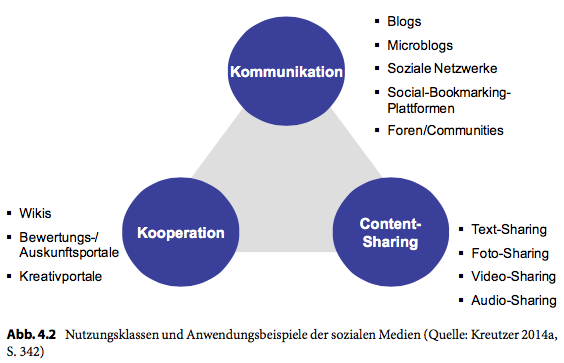
\includegraphics[width=10cm]{kapitel/gruppe1_2/bilder/nutzungsklassen}
	\caption{Hörsaal-Finder der Uni Hohenheim}
	\label{fig_livenavi}
\end{figure}
